%\documentclass[iop,revtex4,apj]{emulateapj}
\documentclass[iop,revtex4]{emulateapj_mod}
\usepackage{natbib}
\usepackage{amsfonts}
\usepackage{amssymb}
\usepackage[printonlyused]{acronym}
\usepackage{amsmath,amsthm}
\usepackage{enumerate}
\usepackage{amsmath, amssymb, mathrsfs}
\usepackage{rotate}
\usepackage{lscape}

\begin{document}
%Title Page: The first page of your report should be the signed Pre-lab Discussion page that was the first page of your lab manual.
\title{Brownian Motion in Cells}
\author{Jung Lin (Doris) Lee}
 \begin{abstract}
 In this lab, we investigate 
 Einstein's prediction 
%Abstract: This should be a brief (100 words) statement of the experiment (what is it?) and your conclusions (what did you do with it?). Be sure to include your final results, along with their associated errors.
 \end{abstract}
 \nocite{*}

%\begin{figure}[h]
%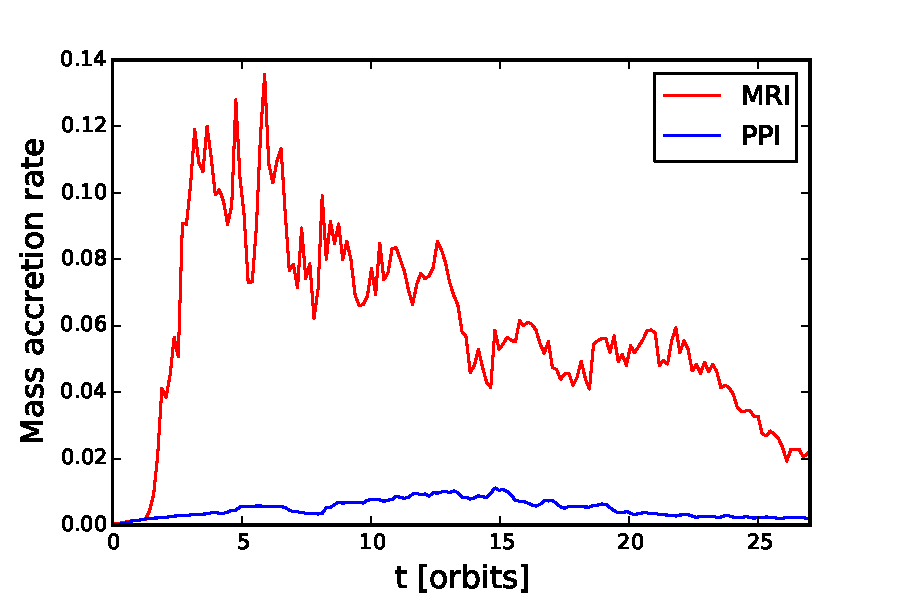
\includegraphics[width=0.45\textwidth,bb=0 0 30 30]{plots/mass_accretion.pdf}
%\caption{The mass accretion rate onto the inner boundary that results from the instabilities.}
%\label{mass_accretion}
%\end{figure}
\section{Introduction}\label{sec:intro}
\par %Introduction: This should describe the physics and give an overview of what you are going to do. Aim to answer the questions: Why would someone want to do this experiment? What is gained?
\section{Theory}\label{sec:theory}
\par 
%Theory: Include the working equations that you will be using but do not include lengthy derivations (such as the Compton or Rutherford formulas) unless specifically asked.where the equations come from and what they are dependent on, (assumptions, conservation laws, etc.), cite reference 
\section{Apparatus and Procedure}\label{sec:ap}
%Apparatus and Procedure: You should have enough detail so that one familiar with physics but not with the particular experiment at hand could reproduce your experiment if necessary. A block diagram of the equipment is essential here—this should be your own, and not copied out of a book or lab manual. Explain the major pieces of equipment and what they do, but do not overwhelm your reader with details here!
\section{Analysis}\label{sec:analysis}
%Analysis:  the calculations that the lab manual asks you to do are supposed to act as a guide to your analysis, and not as a series of separate calculations. agree with prediction? error analysis? source of error, uncertainty?  
\section{Conclusion}\label{sec:conclusion}
%findings, future improvement? 
 
\acknowledgments
\section*{Acknowledgments}
I am sincerely thankful for support from Professor Harmut Haeffner, Kam-Biu Luk, Don Orlando, and my lab partner Xiyue Wang for contributing to successful completion of this lab.

\bibliography{bibdatabase}
%Raw Data: You must include the data that you took in lab in an appendix; the data should be clear enough so that someone could look at it and determine what you measured and how you measured it. You should be keeping a lab notebook, so simply photocopy all relevant pages. Your report should include all of the listed sections, along with the signed Pre-lab and Mid–Lab Discussion sheets.
\end{document}


